% DO NOT CHANGE THIS SEGMENT
% vvvvvvvvvvvvvvvvvvvvvvvvvvvvvvvvvvvvvvvvv
\documentclass[10pt,twocolumn,twoside,a4paper]{article}
% * <rbatzing@gmail.com> 2017-12-11T08:03:48.862Z:
%
\usepackage{mathspec}
\usepackage{polyglossia}
%\setdefaultlanguage[numerals=thai]{thai}
\setdefaultlanguage{thai}
\setotherlanguage{english}
\setmainfont{FreeSerif}
\setsansfont{FreeSerif}
\setmonofont[Scale=1.25,Numbers={Monospaced,Lining},Color=003366]{FreeSerif}
\newfontfamily{\thaifonttt}[Scale=1.25,Numbers={Monospaced,Lining},Color=003366]{FreeSerif}
\setmathsfont(Digits,Latin,Greek){FreeSerif}
\newfontfamily{\thaifont}[Script=Thai,Scale=1.2]{FreeSerif}
\XeTeXlinebreaklocale "th"
\hyphenation{sledge-ham-mer}
%%%%
\usepackage{url}
\usepackage{hyperref}
\usepackage{authblk}
\usepackage{graphicx}
\usepackage{algorithm}
\usepackage{algorithmicx}
\usepackage{algpseudocode}
\usepackage{array}
\usepackage{stfloats}
\usepackage{ntheorem}
\usepackage{listings}
\usepackage{datetime}
\newtheorem{hyp}{สมมติฐานที่}
\gdef\gb{\hfil\penalty -1000}
\usepackage{listings}
\usepackage{titling}
\usepackage[usenames,dvipsnames,svgnames]{xcolor}
%^^^^^^^^^^^^^^^^^^^^^^^^^^^^^^^^^^^^
%%%%%%%%%%%%%%%%%%%%%%%%%%%%%%
% Title and Author
% Change for each document
\title{Choose an appropriate title that uses less than 250 characters}
\author{Student 1 (id number)\and
Student 2 (id number)}%
\date{สาขาวิชาวิทยาการคอมพิวเตอร์ คณะวิทยาศาสตร์\\
    มหาวิทยาลัยพายัพ จังหวัดเชียงใหม่ 50000\\
    ประเทศไทย}
%%vvvvvvvvvvvvvvvvvvvvvvvvvvvvvvvvvvvvvvvv
% Document settings DO NOT CHANGE
\setlength{\droptitle}{-1.2in}% First page to the top
\providecommand{\keywords}[1]{\noindent\textbf{\textit{Keywords---}} #1}
\bibliographystyle{IEEEtran}% IEEE reference style used
\pagestyle{myheadings}
\markboth{\hfill\thetitle}{File: \jobname:\ Compiled: \today \currenttime\hfill}
\linespread{1.5}% linespace for Thai docs
\setlength{\columnsep}{1cm}
\setlength{\columnwidth}{8cm}
\newcounter{cf}
\newfloat{code}{h}{cf}
\floatname{code}{ตัวอย่างโค้ดที่}
\floatname{algorithm}{ขั้นตอนวิธีที่}
\floatstyle{plaintop}
\restylefloat{code}
\restylefloat{table}
\floatstyle{plain}
\restylefloat{figure}
\lstset{firstline=1,numbers=left,
numbersep=7pt,frame=shadowbox,
keywordstyle=\color{DarkGreen},
basicstyle=\footnotesize,
xleftmargin=20pt,xrightmargin=10pt,
rulesepcolor=\color{DarkBlue},
backgroundcolor=\color{LightYellow}}
%%^^^^^^^^^^^^^^^^^^^^^^^^^^^^^^^^^^^^
%%%%%%%%%%%
\begin{document}
\thispagestyle{empty}%
\maketitle

\begin{abstract}
The Abstract summarizes the research project in less than 2,500 characters.
\end{abstract}

\bigskip
\keywords{Keyword1, keyword2, keyword3}

\section{บทนำ}
\label{introduction}
Introduction defines and describes the research question you are trying to answer.

\section{ระเบียบวิธี}
\label{methodology}
Methodology describes the methods and technology did you use to do this research


\section{ผลการวิจัย}
\label{results}
Results provide tables and graphs of your results and describe the key findings

\begin{table}[htb]
\caption{A list of textbooks used for the course}
\label{textbookList}
\medskip
\centering
\small
\begin{tabular}{cr}
\textbf{Author} & \textbf{Pages} \\
1 &	5.333333333 \\
2 &	10.66666667 \\
3 &	16.00000000 \\
4 &	21.33333333 \\
5 &	26.66666667 \\
\end{tabular}
\end{table}

This is the text of my paper as seen in Figure \ref{fig_graph1}.

\begin{figure}[htb]
\centering
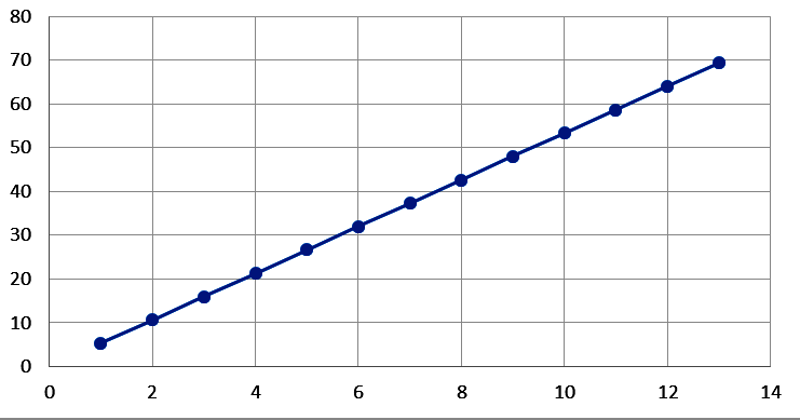
\includegraphics[width=2.5in]{img/graph1.png}
\caption{Time series study}
\label{fig_graph1}
\end{figure}

\section{ข้อสรุป}
\label{conclusion}
Conclusion summarizes your findings and recommends the best answer for your research questions

% use section* for acknowledgment
\section*{คำกล่าวขวัญ}
\label{Acknowledgment}
The authors would like to thank their students for their feedback and insights gained while using this to create their papers.


% references section
\bibliography{classrefs}
\vfill
\end{document}
